%This is a LaTeX template for homework assignments
\documentclass{article}
\usepackage[utf8]{inputenc}
\usepackage{amsmath}
\usepackage{amssymb}
\usepackage{graphicx}
\usepackage{float}
\usepackage{multibibliography}
\begin{document}

\section*{CV Homework 6}{}
Name: Qiang Fu
\\Date: November 26th 2019

\subsection*{Introduction} 
\par
Optical flow, according to the definition in the lecture notes, is a vector field in the image that represents a projection of the image motion field, along the direction of image gradient\cite{ref1}. And the optical flow can be solved under some additional assumptions. This homework is to implement one of the optical flow estimating methods and evaluate the results.
\subsection*{Theories for the algorithm}
\par
According to the lecture notes, the motion field is defined as the 2D vector field of velocities of the image points, included by relative 3D motin between the view camera and the observed scene. It can also be interprated as the projection of 3D velocity field on the image plane.\cite{ref1} And to derive the relationship between the image points and the motion field we need to make an assumption
\begin{equation}
\frac{dI}{dt}=0
\end{equation}
where we see $I(c,r,t)$ the intensity as a function of image coordinates $c, r$ and time frame $t$. And the assumption we made is basicly that the intensity of a specific 3D point's projection on 2D image plane is time invariant. Then we have
\begin{equation}
\frac{dI}{dt}=\frac{\delta I}{\delta c}\frac{dc}{dt}+\frac{\delta I}{\delta r}\frac{dr}{dt}+\frac{\delta I}{\delta t}=0
\end{equation}
where $\frac{\delta I}{\delta c}$ and $\frac{\delta I}{\delta r}$ represent the spatial intensity gradient, $\frac{\delta I}{\delta t}$ represents the temporal intensity gradient. And $\begin{bmatrix}\frac{dc}{dt}\\\frac{dr}{dt}\end{bmatrix}$ is the motion vector $\begin{bmatrix}v_c\\v_r\end{bmatrix}$. Thus we can rewrite Eq.2 as 
\begin{equation}
(\triangledown I)^Tv+I_t=0
\end{equation}
where $\triangledown I$ is called image intensity gradient. we can easily find that Eq.3 can only determine motion flow component in the direction of the intensity gradient. And this component is called optical flow. However only using the Eq.3 we can't reconstruct the optical flow because we have only 1 equation with 2 unknowns. Then we need more constraints to solve the optical flow.
\par 
The assumption I use in this homework is called image brightness change constancy assumption. The main idea of this assumption is that while objects are in motion, we can assume both spatial and temporal image brightness change to be constant, i.e., image brightness change rates in c, r, and t are constant.\cite{ref1} 
\begin{equation}
\frac{d^2I}{dtdc}=0,\frac{d^2I}{dtdr}=0,\frac{d^2I}{dtdt}=0
\end{equation}
Then for Eq.3 we can have
\begin{align}
\begin{split}
v_cI_c+v_rI_r+I_t&=0\\
v_cI_{cc}+v_rI_{rc}+I_{tc}&=0\\
v_cI_{cr}+v_rI_{rr}+I_{tr}&=0\\
v_cI_{ct}+v_rI_{rt}+I_{tt}&=0
\end{split}
\end{align}
And we can rewrite Eq.5 in matrix form
\begin{equation}
Av=b
\end{equation}
where $A = \begin{bmatrix}I_c&I_r\\I_{cc}&I_{cr}\\I_{rc}&I_{rr}\\I_{tc}&I{tr}\end{bmatrix},b = -\begin{bmatrix}I_t\\I_{ct}\\I_{rt}\\I_{tt}\end{bmatrix}$
We can solve optical flow vector $v$ using least squares method by minimizing $\left\|Av-b\right\|_2^2$, then 
\begin{equation}
x=(A^TA)^{-1}A^Tb
\end{equation}
\par
To implement the method mentioned above, we need to compute the iamge derivatives first. And normally we have two methods. The fisrt one is called numerical method. This method is simple but very sensitive to the noise\cite{ref1}. The second method is called surface fitting method, and it is also the method I use for this homework. We chose a $5\times5\times5$ window, and we can see the points in this window locate on a hypersurface $I(c,r,t)$. And by least squares method, we can get the surface and reduce the influence of noise.
\begin{align}
\begin{split}
I(c,r,t)=&a_1+a_2c+a_3r+a_4t+a_5c^2+a_6cr\\
&+a_7r^2+a_8rt+a_9t^2+a_{10}ct+a_{11}c^3+a_{12}c^2r\\
&+a_{13}cr^2+a_{14}r^3+a_{15}r^2t+a_{16}rt^2+a_{17}t^3\\
&+a_{18}c^2t+a_{19}ct^2+a_{20}crt
\end{split}
\end{align}
And we ca rewrite Eq.8 in matrix form 
\begin{equation}
Da=J
\end{equation}
where $a=(a_1,a_2,\dots,a_{20})^T$, $D=\begin{bmatrix}1&c_1&r_1&t_1&\dots&c_1r_1t_1\\
1&c_2&r_1&t_1&\dots&c_2r_1t_1\\
\vdots&\vdots&\vdots&\vdots& &\vdots\\
1&c_k&r_1&t_1&\dots&c_kr_1t_1\\
1&c_1&r_2&t_1&\dots&c_1r_2t_1\\
1&c_2&r_2&t_1&\dots&c_2r_2t_1\\
\vdots&\vdots&\vdots&\vdots& &\vdots\\
1&c_k&r_2&t_1&\dots&c_kr_2t_1\\
\vdots&\vdots&\vdots&\vdots& &\vdots\\
1&c_1&r_k&t_k&\dots&c_1r_kt_k\\
1&c_2&r_k&t_k&\dots&c_2r_kt_k\\
\vdots&\vdots&\vdots&\vdots& &\vdots\\
1&c_k&r_k&t_k&\dots&c_kr_kt_k\\
\end{bmatrix}$\\
and $J=\begin{bmatrix}
I(c_1,r_1,t_1)\\
I(c_2,r_1,t_1)\\
\vdots\\
I(c_k,r_k,t_k)
\end{bmatrix}$
We can use least squares method to solve $a$ by minimizing $\left\|Da-J\right\|^2$. And 
\begin{equation}
a=(D^TD)^{-1}D^TJ
\end{equation}
By using the relative coordinates instead of actual coordinates we can make the $D$ matrix same for all the points.

\subsection*{Results}
\par
The results are as following 
\begin{figure}[H]
\centering
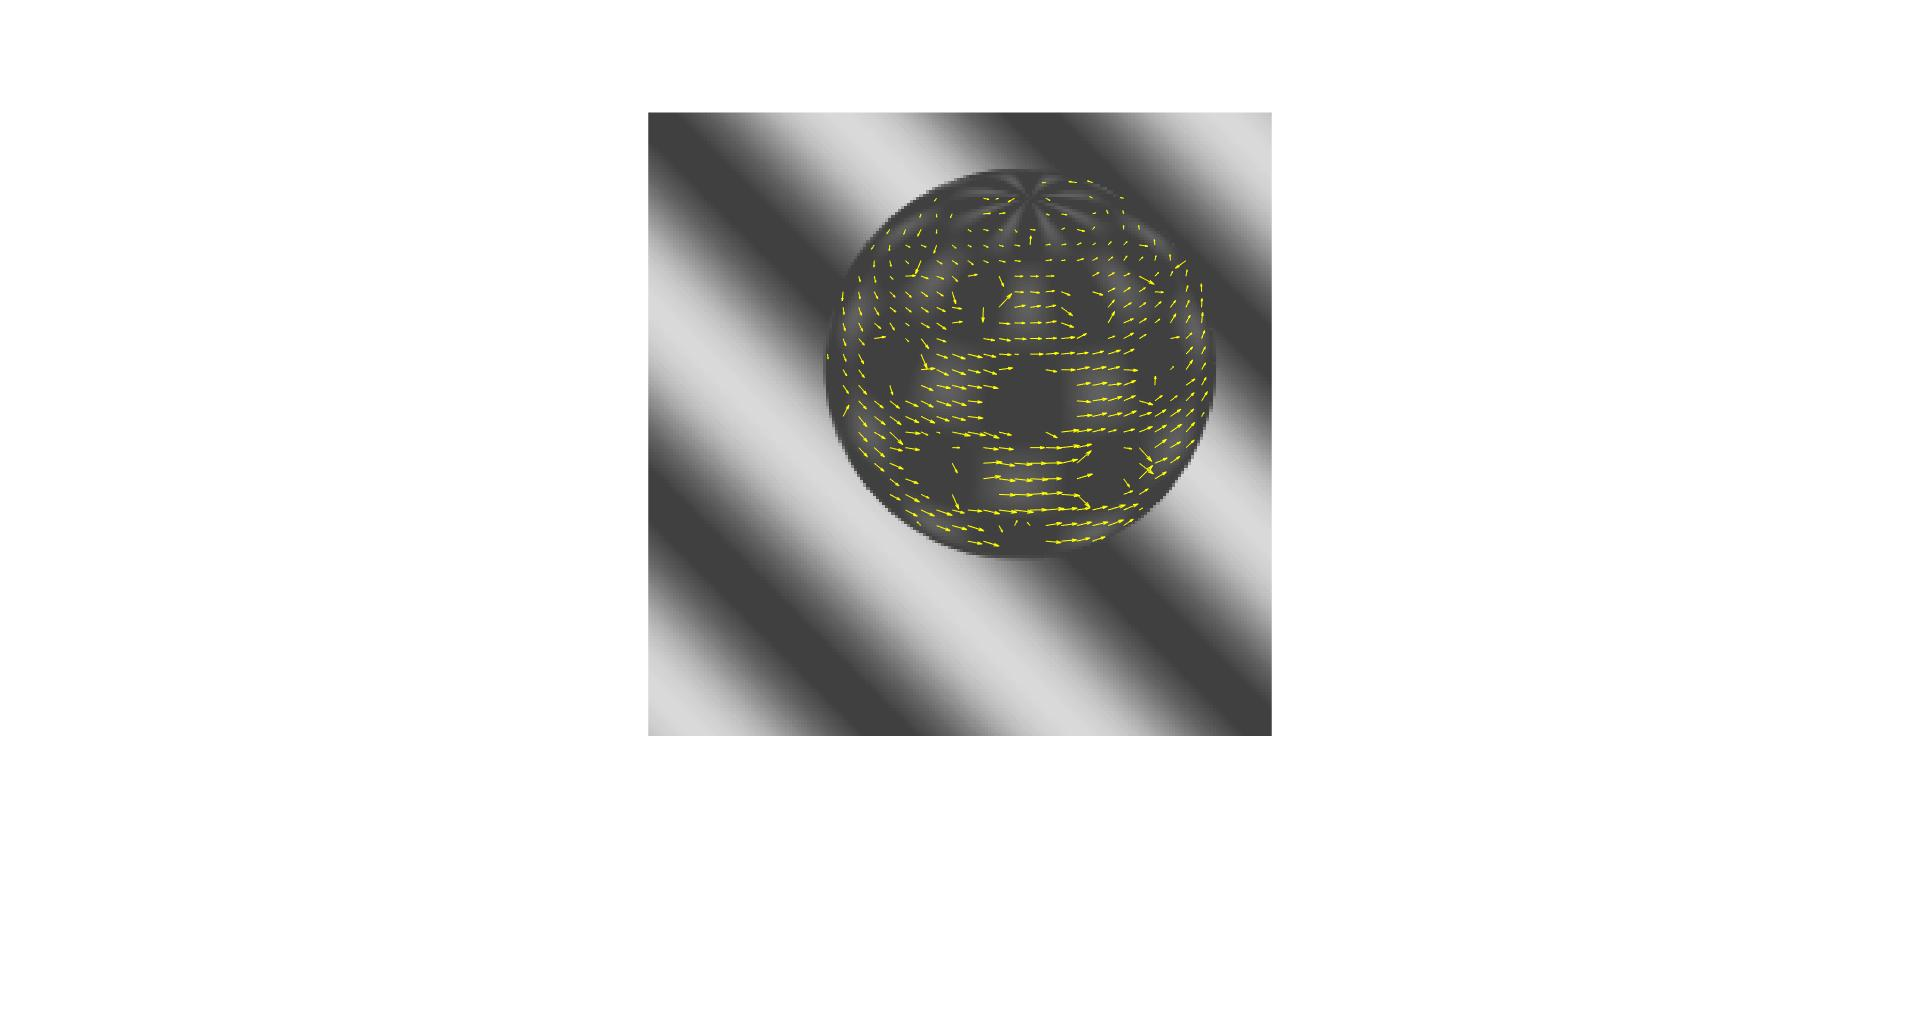
\includegraphics[scale=0.2]{1.jpg}
\caption{optical flow of sequence 1}
\label{fig:label}
\end{figure}
This is the optical flow of sequence 1. Form figure.1 we can find that for most of the points the optical flows seem correct, however there are still some points with incorrect optical flow. I think this is because the optical flow is the motion's component that parallel with the image gradient, so if the iamge spatial gradient is influenced by iamge noise, the optical flow will als be influenced.
\par 
The result of the second sequence is as following 
\begin{figure}[H]
\centering
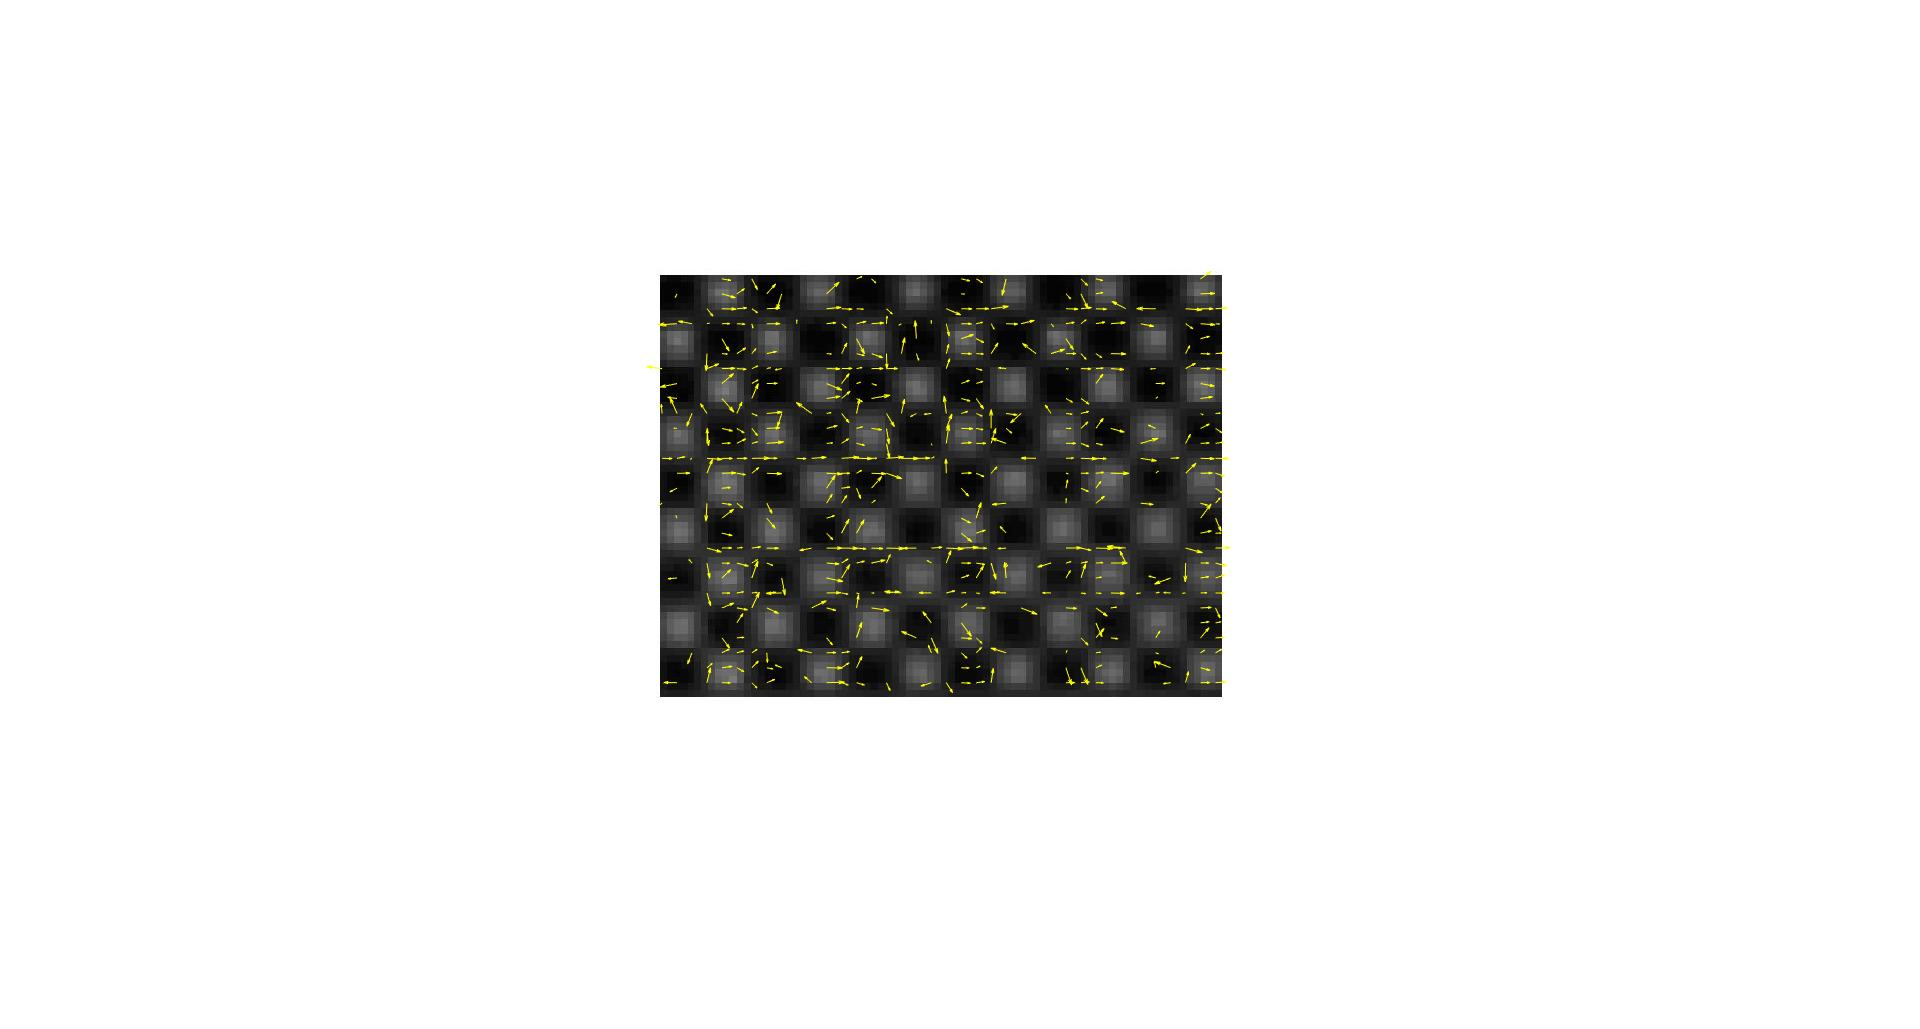
\includegraphics[scale=0.2]{2.jpg}
\caption{optical flow of sequence 2}
\label{fig:label}
\end{figure}
We can find that the result contains much more error than the first sequence.
\subsection*{Summary and conclusion}
\par
In this homework, we made two important assumptions, the first one is the iamge brightness constancy assumption and the second one is the image brightness change constancy assumption. And based on these assumptions we can set up linear equations to solve the optical flow. And during constructing the linear system, we applied surface fitting method to compute the intensity gradients. From the results we can find that for the first sequence, this method works well, however for the second sequence, the result contains much error.
\newpage
\begin{thebibliography}{}  
\bibitem{ref1}Qiang Ji. RPI ECSE 6650 Computer Vision, Lecture Notes: Motion. URL:https://www.ecse.rpi.edu/\~qji/CV/motion2.pdf. Last visited on 2019/11/26.
\end{thebibliography}
\end{document}

\end{document}